% 翻译:SI
% 未校对!

\chapter{Maxwell关系}
\label{chap7}

\section{Maxwell关系}
\label{sec7.1}
\ref{sec3.9}节\mpar{原文为\ref{sec3.6}节,根据内容来看应该是\ref{sec3.9}节。这里进行了修改。}讨论了绝热压缩率、热膨胀系数、摩尔热容等热力学量的物理意义。它们都具有$(\partial X / \partial Y)_{Z, W}$的形式,式中字母表示热力学广延量或强度量。一般的热力学系统有许多热力学量,从而可以构造大量这样的导数。但是众多的导数量之间存在羁绊,其中只有一小部分是独立的,其余的量可以用这一小部分表示。自然,这些关系可以大大简化热力学分析。并且我们不需要特意记忆公式\mpar{比如“{\bf G}ood {\bf P}hysicists {\bf H}ave {\bf S}tudied {\bf U}nder {\bf V}ery {\bf F}ine {\bf T}eachers”什么的……\sout{来自热统课的惨痛回忆}\ \sout{\ref{sec7.2}节有首字母相同的另一句话} }。 下面介绍在热力学计算过程中用到的简单、直接推导这些关系的方法,也就是本章的主题。

首先说明这些导数量之间“羁绊”的存在性,考虑\eqref{equ3.70}与\eqref{equ3.71}式:
\begin{align}
	\frac{\partial^2 U}{\partial S \partial V} &= \frac{\partial^2 U}{\partial V \partial S}, \label{equ7.1} \\
	-\left( \frac{\partial P}{\partial S} \right)_{V, N_1, N_2} &= \left( \frac{\partial T}{\partial V} \right)_{S, N_1, N_2}. \label{equ7.2}
\end{align}
上式是导数量的“羁绊”——称为{\it Maxwell 关系 (Maxwell relations)}——的源头,亦即,导数量之间的依赖关系源自基本方程(在不同表象下)的混合导数不依赖于求导次序。

某一热力学量依赖于$(t + 1)$个自变量,从而有$t(t + 1)/2$种不同的混合偏导数,因此每一热力学量对应$t(t + 1)/2 = 3$个Maxwell关系。

单组分简单系统的内能的自变量有$3$个,即$t = 2$,从而有$(2 \cdot 3)/2$个混合偏导数:
\[
	\frac{\partial^2 U}{\partial S \partial V} = \frac{\partial^2 U}{\partial V \partial S}, \quad \frac{\partial^2 U}{\partial S \partial N} = \frac{\partial^2 U}{\partial N \partial S}, \quad \frac{\partial^2 U}{\partial V \partial N} = \frac{\partial^2 U}{\partial N \partial V}.
\]
单组分简单系统的Maxwell列成下表。其中第一列是混合求导的热力学量,第二列是混合求导对应的两个(独立)自变量,第三列是相应的Maxwell关系。\ref{sec7.2}节提供了一种辅助记忆这些关系的图像法。\ref{sec7.3}节举例说明如何利用这些关系解决热力学问题。

\begin{align}
	&U \quad &S, V \quad & \left( \frac{\partial T}{\partial V} \right)_{S, N} =& -\left( \frac{\partial P}{\partial S} \right)_{V, N} \label{equ7.3} \\
	&dU = TdS - PdV + \mu dN \quad & S, N \quad & \left( \frac{\partial T}{\partial N} \right)_{S, V} =& \left( \frac{\partial \mu}{\partial S} \right)_{V, N} \label{equ7.4} \\
	&\phantom{dU = TdS - PdV + \mu dN \quad} & V, N \quad & -\left( \frac{\partial P}{\partial N} \right)_{S, V} &= \left( \frac{\partial \mu}{\partial V} \right)_{S, N} \label{equ7.5}
\end{align}
————————————————————————————————
\begin{align}
	&U[T]\equiv F & T, V \quad & \left(\frac{\partial S}{\partial V} \right)_{T, N} &= \left( \frac{\partial P}{\partial T} \right)_{V, N} \label{equ7.6} \\
	&dF = -SdT - PdV + \mu dN \quad & T, N \quad & -\left(\frac{\partial S}{\partial N}\right)_{T, V} &= \left(\frac{\partial \mu}{\partial T} \right)_{V, N} \label{equ7.7} \\
	&\phantom{dF = -SdT - PdV + \mu dN \quad} & V, N \quad & -\left( \frac{\partial P}{\partial N} \right)_{T, V} &= \left( \frac{\partial \mu}{\partial V} \right)_{T, N} \label{equ7.8}
\end{align}
————————————————————————————————
\begin{align}
	& U[P] \equiv H \quad & S, P \quad & \left( \frac{\partial T}{\partial P} \right)_{S, N} &= \left( \frac{\partial V}{\partial S} \right)_{P, N} \label{equ7.9} \\
	&dH = TdS + VdP + \mu dN \quad & S, N \quad & \left( \frac{\partial T}{\partial N} \right)_{S, P} &= \left( \frac{\partial \mu}{\partial S} \right)_{P, N} \label{equ7.10} \\
	&\phantom{dH = TdS + VdP + \mu dN \quad} & P, N \quad & \left(\frac{\partial V}{\partial N} \right)_{S, P} &= \left( \frac{\partial \mu}{\partial P} \right)_{S, N} \label{equ7.11} 
\end{align}
————————————————————————————————
\begin{align}
	& U[\mu] \quad & S, V \quad & \left(\frac{\partial T}{\partial V} \right)_{S, \mu} &= -\left( \frac{\partial P}{\partial S} \right)_{V, \mu} \label{equ7.12} \\
	& dU[\mu] = TdS - PdV - Nd\mu \quad & S, \mu \quad & \left(\frac{\partial T}{\partial \mu} \right)_{S, V} &= -\left( \frac{\partial N}{\partial S} \right)_{V, \mu} \label{equ7.13} \\
	& \phantom{dU[\mu] = TdS - PdV - Nd\mu \quad} & V, \mu \quad & \left(\frac{\partial P}{\partial \mu} \right)_{S, V} &= \left( \frac{\partial N}{\partial V} \right)_{S, \mu} \label{equ7.14}
\end{align}
————————————————————————————————
\begin{align}
	& U[T, P] \equiv G \quad & T, P \quad & -\left( \frac{\partial S}{\partial P} \right)_{T, N} &= \left( \frac{\partial V}{\partial T} \right)_{P, N} \label{equ7.15} \\
	& dG = -SdT + VdP + \mu dN \quad & T, N \quad & -\left( \frac{\partial S}{\partial N} \right)_{T, P} &= \left( \frac{\partial \mu}{\partial T} \right)_{P, N} \label{equ7.16} \\
	& \phantom{dG = -SdT + VdP + \mu dN \quad} & P, N \quad & \left( \frac{\partial V}{\partial N} \right)_{T, P} &= \left( \frac{\partial \mu}{\partial P} \right)_{T, N} \label{equ7.17}
\end{align}
————————————————————————————————
\begin{align}
	& U[T, \mu] \quad & T, V \quad & \left( \frac{\partial S}{\partial V} \right)_{T, \mu} &= \left( \frac{\partial P}{\partial T} \right)_{V, \mu} \label{equ7.18} \\
	& dU[T, \mu] = -SdT - PdV - Nd\mu \quad & T, \mu \quad & \left( \frac{\partial S}{\partial \mu} \right)_{T, V} &= \left( \frac{\partial N}{\partial T} \right)_{V, \mu} \label{equ7.19} \\
	& \phantom{dU[T, \mu] = -SdT - PdV - Nd\mu \quad} & V, \mu \quad & \left( \frac{\partial P}{\partial \mu} \right)_{T, V} &= \left( \frac{\partial N}{\partial V} \right)_{T, \mu} \label{equ7.20}
\end{align}
————————————————————————————————
\begin{align}
	& U[P, \mu] \quad & S, P \quad & \left( \frac{\partial T}{\partial P} \right)_{S, \mu} =& \left( \frac{\partial V}{\partial S} \right)_{P, \mu} \label{equ7.21} \\
	& dU[P, \mu] = TdS + VdP + Nd\mu \quad & S, \mu \quad & \left( \frac{\partial T}{\partial \mu} \right)_{S, P} =& -\left( \frac{\partial N}{\partial S} \right)_{P, \mu} \label{equ7.22} \\
	& \phantom{ dU[P, \mu] = TdS + VdP + Nd\mu \quad} & P, \mu \quad & \left( \frac{\partial V}{\partial \mu} \right)_{S, P} =& -\left( \frac{\partial N}{\partial P} \right)_{S, \mu} \label{equ7.23}
\end{align}
————————————————————————————————

\section{Maxwell关系的辅助记忆图}
\label{sec7.2}
最常用的Maxwell关系可以通过如下的图像辅助记忆\footnote{This diagram was presented  by  Professor Max Born in  1929  in a lecture heard  by  Professor Tisza. 它出现在论文 F. O. Koenig, {\it J. Chem. Phys} {\bf 3}, 29 (1935),  以及 {\bf 56}, 4556 (1972). 另外可见 L T. Klauder,  {\it Am. Journ. Phys}. {\bf 36}, 556 (1968), 并且此期刊中有其他作者提出的一系列变体。},见图\ref{fig7.1}。它由一个正方形以及两条沿对角线指向上的箭头组成。正方形的每条边由热力学量$F, G, H, U$标记,Helmholtz势$F$居最上,其余三者按顺时针方向的字母表顺序排列。左侧的两个顶点是广延量$V, S$, 右侧顶点是强度量$T, P$. (整个顺序可以用`` {\bf V}alid {\bf F}acts and {\bf T}heoretical {\bf U}nderstanding {\bf G}enerate {\bf S}olutions to {\bf H}ard {\bf P}roblems ''来记忆)

{
	\centering
	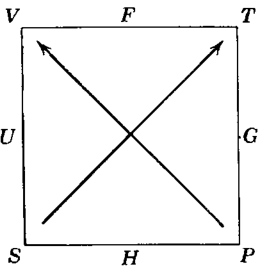
\includegraphics{fig7_1.png}
	\figcaption{热力学正方形}
	\label{fig7.1}
}

位于正方形边上的四个热力学势是它们附近的两个独立变量的函数。例如$U$是$V, S$的函数;$F$是$V, T$的函数;$G$是$T, P$的函数;等等。所有热力学势还是摩尔数$N$的函数,这在图中并未显示。

各热力学势的微分表达式中每一项的正负号由对角线箭头辅助记忆。如果箭头背离自变量,则该项是正的;而箭头指向自变量则表明该项为负。结合如下等式观察图像不难掌握这一方法:
\begin{align}
	dU &= TdS - PdV + \sum_k \mu_k dN_k \label{equ7.24} \\
	dF &= -SdT - PdV + \sum_k \mu_k dN_k \label{equ7.25} \\
	dG &= -SdT + VdP + \sum_k \mu_k dN_k  \label{equ7.26} \\
	dH &= TdS + VdP + \sum_k \mu_k dN_k  \label{equ7.27}
\end{align}

Maxwell关系可以按如下方法从图中读取。只考虑正方形顶点的量,不难看出等式的图的关系:
\begin{equation}
	\left( \frac{\partial V}{\partial S} \right)_P = \left( \frac{\partial T}{\partial P} \right)_S \quad (N_1, N_2, \dots \text{为常数})
\label{equ7.28}
\end{equation}
{
	\centering
	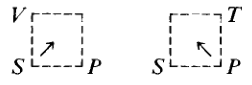
\includegraphics[scale=0.7]{equ7_28.png}
}

把图像顺时针旋转$90^\circ$, 从新图像读出:
\begin{equation}
	\left( \frac{\partial S}{\partial P} \right)_T = -\left( \frac{\partial V}{\partial T} \right)_P \quad (N_1, N_2, \dots \text{为常数})
\label{equ7.29}
\end{equation}
{
	\centering
	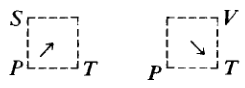
\includegraphics[scale=0.7]{equ7_29.png}
}

上图中两个箭头指向不同意味着上式有负号。再旋转图像两次可以得到其余两个Maxwell关系:
\begin{align}
	\left( \frac{\partial P}{\partial T} \right)_V &= \left( \frac{\partial S}{\partial V} \right)_T \quad (N_1, N_2, \dots, \text{为常数}) \label{equ7.30}\\
	\left( \frac{\partial T}{\partial V} \right)_S &= - \left( \frac{\partial P}{\partial S} \right)_V \quad (N_1, N_2, \dots \text{为常数}) \label{equ7.31}
\end{align}
以上四式即为最常用的Maxwell关系。

这种辅助记忆图还可以推广到变量$S, V$之外的其它变量。例如考虑经Legendre变换后的$S, N_j$, 相应的图像变为\ref{fig7.2}(a). 连接$N_j$与$\mu_j$的箭头与原图中连接$V, P$的箭头方向相反,因为$\mu_j$的地位与$-P$相同。从该图中可以读出\eqref{equ7.4}, \eqref{equ7.7}, \eqref{equ7.13}和\eqref{equ7.19}式。其它Legendre变换的辅助图类似,一般情况见\ref{fig7.2}(b).

{
	\centering
	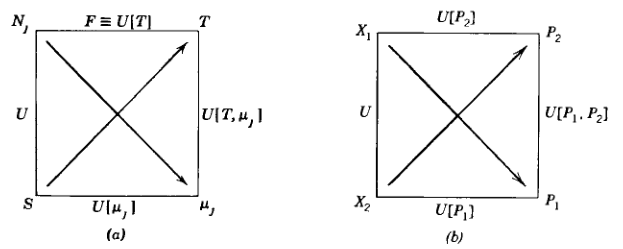
\includegraphics[scale=0.8]{fig7_2.png}
	\figcaption{}
	\label{fig7.2}
}

\subsection*{习题}


\section{一种导数约化的步骤}
\label{sec7.3}
在热力学的实际应用中,经常需要计算偏导数以分析实验过程。例如,分析单组分系统在恒容条件下压强与温度的变化关系,显然有
\begin{equation}
	\rd T = \left( \frac{\partial T}{\partial P} \right)_{V, N} \rd P.
\label{equ7.32}
\end{equation}
然后就是要计算偏导数$(\partial T / \partial P)_{V, N}$. \ref{sec7.4}节会讨论一系列类似问题。这种偏导数量都有共同特点,求导过程中的摩尔数$N$均不变,并且既含有广延量又有强度量。{\it 所有这些导数当中只有三个是独立的,任意选定作为基的三个量之后,其余的偏导数都可以用这三者表示。} 通常选择$c_P, \alpha, \kappa_T$作为基。

$c_P, \alpha, \kappa_T$暗示着用Gibbs表象,因为在该表象下三个量简单表述为$\partial^2 g / \partial T^2, \partial^2 g / \partial T \partial P$以及$\partial^2 g / \partial P^2$;它们又分别等于$-c_P / T, v\alpha$以及$-v \kappa_T$. 在系统摩尔数不变的情况下,其余的二阶导数都依赖于它们。

{\it 所有一阶导数(既包括对广延量、也包括对强度量求导)可以表为Gibbs势二阶偏导数量的函数,例如上面的$c_P, \alpha, \kappa_T$就构成一组完备集(在摩尔数不变的情况下)。}

“导数约化”的过程原则上十分直接,只需要把熵$S$替换成$-\partial G / \partial T$, $V$换成$\partial G / \partial P$,接着原始偏导数量用$G$对$T, P$的二阶混合导数表示出来即可。但实际上这么干会相当复杂。

学过热力学的人的一个基本技能是熟练掌握“导数约化”技术——将任意偏导数量用已知的偏导数基表示。为此,我们提出一种基于上一节“正方形记忆图”的方法,并且整理成了按部就班的套路。只有进行大量练习才能真正掌握。

以下假设求导过程的摩尔数均不变。要将给定的导数表示为$c_P, \alpha, \kappa_T$的函数。之后会用到如下微积分恒等式(见附录A):
\begin{equation}
	\left( \frac{\partial X}{\partial Y} \right)_Z = 1 \Big/ \left(\frac{\partial Y}{\partial X} \right)_Z 
\label{equ7.33}
\end{equation}
以及
\begin{align}
	\left( \frac{\partial X}{\partial Y} \right)_Z &= \left( \frac{\partial X}{\partial W} \right)_z \Bigg/ \left( \frac{\partial Y}{\partial W} \right)_Z \label{equ7.34} \\
	\left( \frac{\partial X}{\partial Y} \right)_Z &= - \left( \frac{\partial Z}{\partial Y} \right)_X \Bigg/ \left( \frac{\partial Z}{\partial X} \right)_Y \label{equ7.35}
\end{align}

接着,按照顺序执行下列运算:

\begin{enumerate}
\item {\bf 如果导数中含有势函数,那么把它们化到分子中,并且利用热力学正方形暗示的等量关系(\eqref{equ7.24} - \eqref{equ7.27}式)将它消去。}
\paragraph{例} 化简导数$(\partial P / \partial U)_{G, N}$.
\begin{align}
	\left( \frac{\partial P}{\partial U} \right)_{G, N} &= \left[ \left( \frac{\partial U}{\partial P} \right)_{G, N} \right]^{-1} \tag{by \eqref{equ7.33} } \\
	&= \left[ T \left( \frac{\partial S}{\partial P} \right)_{G, N} - P \left( \frac{\partial V}{\partial P} \right)_{G, N} \right]^{-1} \tag{by \eqref{equ7.34} }  \\
	&= \left[ -T \left( \frac{\partial G}{\partial P} \right)_{S, N} \Bigg/ \left( \frac{\partial G}{\partial S} \right)_{P, N} + P \left( \frac{\partial G}{\partial P} \right)_{V, N} \Bigg/ \left( \frac{\partial G}{\partial V} \right)_{P, N} \right]^{-1} \tag{by \eqref{equ7.35} } \\
	&= \left[ -T \frac{-S (\partial T / \partial P)_{S, N} + V}{-S (\partial T / \partial S)_{P, N}} + P \frac{-S(\partial T / \partial P)_{V, N} + V}{-S (\partial T / \partial V)_{P, N}} \right]^{-1} \tag{by \eqref{equ7.26} }
\end{align}
经过处理后的表达式不含任何势函数,只含有导数。然后按如下步骤处理导数量。
\item {\bf 如果导数中含有化学势,那么把它化到分子中,再利用Gibbs-Duhem关系}$\rd \mu = -s \rd T + v\rd P${\it 消去它。}

\paragraph{例} 化简$( \partial \mu / \partial V)_{S, N}$.

\[
	\left( \frac{\partial \mu}{\partial V} \right)_{S, N} = -s \left( \frac{\partial T}{\partial V} \right)_{S, N} + v \left( \frac{\partial P}{\partial V} \right)_{S, N}
\]
\item {\bf 如果导数中含有熵,则将它化到分子。如果正方形记忆图中的四个Maxwell关系可以消去这个熵的导数,则调用它消去。如果Maxwell关系不能消去熵,那么利用\eqref{equ7.34}式(令其中的$w = T$)凑出$\partial S / \partial T$, 这样分子就能表示为热容$c_v$或$c_P$的函数。}

\paragraph{例} 考虑第1步出现的导数$(\partial T / \partial P)_{S, N}$:
\begin{align}
	\left( \frac{\partial T}{\partial P} \right)_{S, N} &= - \left( \frac{\partial S}{\partial P} \right)_{T, N} \Bigg/ \left( \frac{\partial S}{\partial T} \right)_{P, N} \tag{by \eqref{equ7.35}} \\
	&= \left( \frac{\partial V}{\partial T} \right)_{P, N} \Bigg/ \frac{N}{T} c_P \tag{by \eqref{equ7.29}}
\end{align}

\paragraph{例} 考虑导数$(\partial S / \partial V)_{P, N}$, 利用Maxwell关系$(\partial S / \partial V)_{P, N} = (\partial P / \partial T)_{S, N}$ (\eqref{equ7.28}式)不能消去熵,因此不调用Maxwell关系,而是凑出$\partial S / \partial T$:
\begin{equation}
	\left( \frac{\partial S}{\partial V} \right)_{P, N} = \frac{(\partial S / \partial T)_{P, N}}{(\partial V / \partial T)_{P, N}} = \frac{(N / T) c_P}{(\partial V / \partial T)_{P, N}} \tag{by \eqref{equ7.34}}
\end{equation}
于是将导数化成了不含势函数也不含有熵的形式,只包括$V, P, T$(当然还有$N$)。
\item {\bf 将$V$化入分子,这样出现的量都能表示为$\alpha$与$\kappa_T$的函数。}

\paragraph{例} \begin{equation}
	\left( \frac{\partial T}{\partial P} \right)_{V, N} = -\left( \frac{\partial V}{\partial P} \right)_{T, N} \Bigg/ \left( \frac{\partial V}{\partial T} \right)_{P, N} = \frac{\kappa_T}{\alpha} \tag{by \eqref{equ7.35}}
\end{equation}

\item {\bf 最初给定的导数经以上步骤已经化成了用$c_v, c_P, \alpha, \kappa_T$表示的形式。恒容热容可以用下式消去:}
\begin{equation}
	c_v = c_P - \frac{Tv\alpha^2}{\kappa_T}
\label{equ7.36}
\end{equation}
上式即\eqref{equ3.75}式的变形,它经常被用到,应该牢记。读者也要掌握上式的推导(见习题7.3-2)。
\end{enumerate}

上面导数约化的步骤以单组分系统为例,但也可以推广到多组分系统,只要组分的化学势$\mu_j$不出现在导数中(因为单组分系统的化学势是通过Gibbs-Duhem关系消去的,对于多组分系统而言G-D关系将一种化学势化为了其他化学势)。

\subsection*{习题}

\section{简单应用}
\label{sec7.4}

\section{磁系统的推广}
\label{sec7.5}
